\documentclass[12pt]{article}

\usepackage{amsmath}

\usepackage{graphicx}
\usepackage{subcaption}

\usepackage{placeins}

\usepackage[margin=2.54cm]{geometry}


\usepackage[style=numeric, sorting=none]{biblatex}
\addbibresource{bib_files/Biblio.bib}

%-------------------------- début du document ---------------------------%


\begin{document}

%----------------------------- page de garde ----------------------------%
\fontsize{12pt}{14pt}\selectfont
\begin{figure}[ht]
\vspace{0.3cm}
    \centering
    \begin{subfigure}[b]{0.2\textwidth}
        
\includegraphics[width=\textwidth]{images/Logo_UM.png}
    \end{subfigure}
    \begin{subfigure}[b]{0.2\textwidth}
        
\includegraphics[width=\textwidth]{images/Logo_FDS.png}
    \end{subfigure}
    \begin{subfigure}[b]{0.2\textwidth}
        
\includegraphics[width=\textwidth]{images/Logo_cea.png}
    \end{subfigure}
\end{figure}

% \floatbarrier

\begin{center}
\vspace{1.2cm}
\LARGE{UNIVERSITÉ DE MONTPELLIER}
	
\vspace{0.8cm}
\LARGE{FACULTÉ DES SCIENCES}

\vspace{0.8cm}
\LARGE{ COMMISSARIAT A L'ENERGIE ATOMIQUE ET AUX ENERGIES ALTERNATIVES}
	
\vspace{1.7cm}	
\Large
\textbf{Report of the Alternance program for the Masters second year in Computational Physics}

\vspace{1.3cm}
\normalsize	{Author :}\\
\vspace{.3cm}
\large{\textbf{Nischal Dhungana}}
	
\vspace{1.3cm}
\normalsize	{Under the supervision of :} \\
\vspace{.3cm}
\large
\textbf{Guillame Freychet}

\vspace{1.3cm}
\textbf{June 2024}
\end{center}

%--------------------------- remerciements ------------------------------%
\newpage
\section*{Acknowledgements}

\medskip


%------------------------------ table des matières ----------------------%
\newpage

\tableofcontents


%----------------------------- outline -----------------------------%

\section{Introduction}

\medskip

The continuous miniaturization of microelectronic components, driven by Moore's Law, 
has led to a significant reduction in transistor size and increased chip complexity.
This rapid advancement has presented new challenges in the field of metrology, the science of measurement.
Existing metrology techniques, such as Optical Critical Dimension (OCD) and Critical Dimension Scanning 
Electron Microscope (CDSEM), are reaching their limits in terms of resolution and accuracy as feature sizes
shrink to the nanometer scale.


\begin{figure}[h]
    \centering
    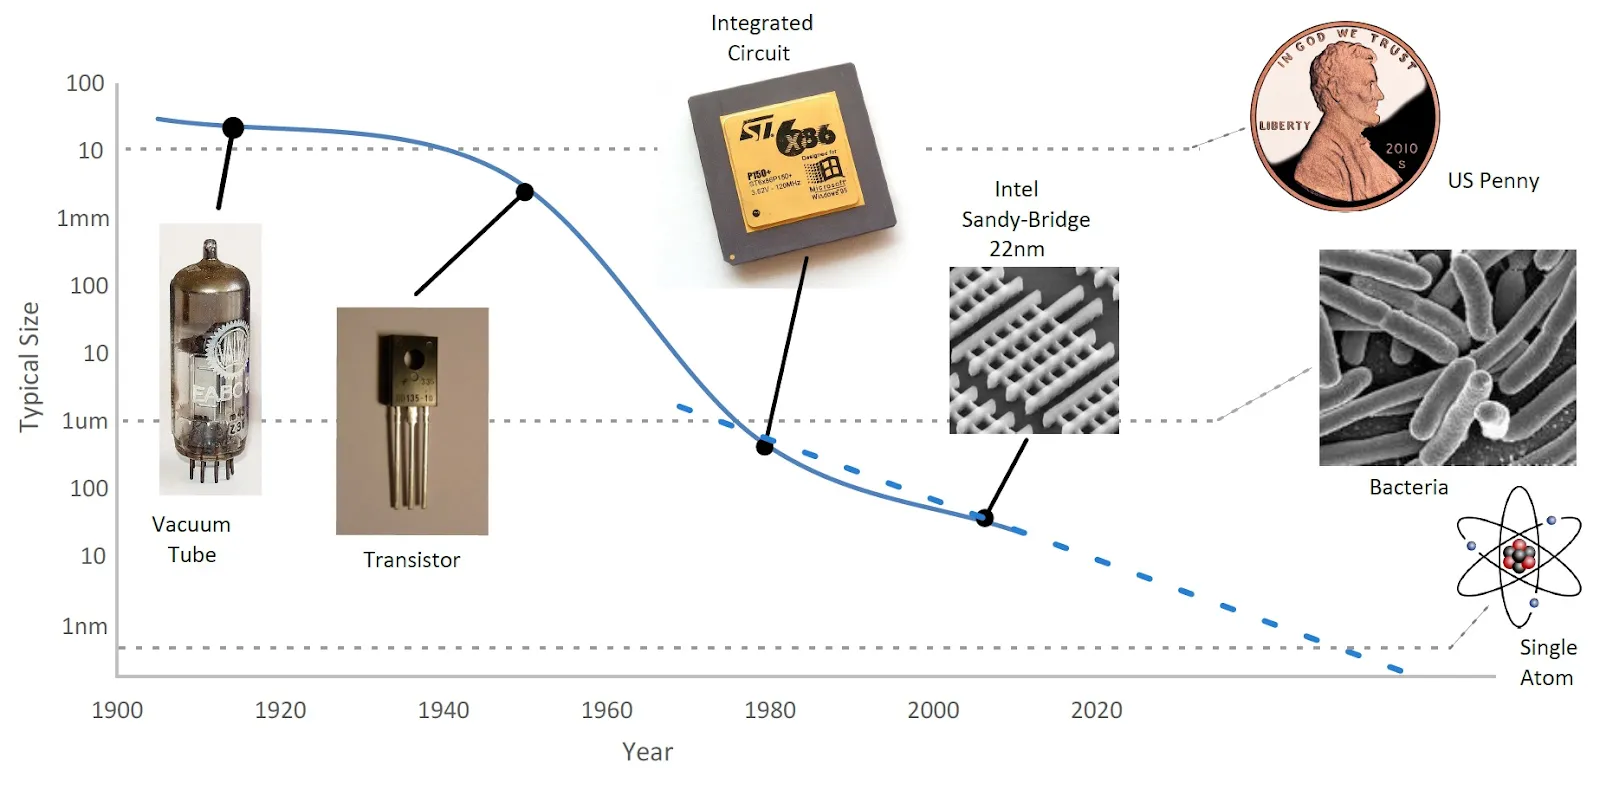
\includegraphics[width=0.8\textwidth]{images/moore's_law.png}
    \caption{Evolution of microelectronics and the need for advanced metrology techniques \cite{moore_law}.}
    \label{fig:evolution_microelectronics}
\end{figure}

\FloatBarrier

To address these challenges, a new metrology technique called Critical Dimension Small Angle X-ray Scattering
(CDSAXS) is being developed. CDSAXS utilizes short-wavelength X-rays $(\lambda \approx 0.05 - 5 nm)$, to probe the internal structure of
materials, providing high-resolution measurements of critical dimensions (CDs) with greater accuracy than
conventional methods. CEA-Leti, a leading research institute in microelectronics, is actively involved in
the development of CDSAXS technology.

\medskip

This work-study project focused on the development of a coherent software for the fit and analysis of CDSAXS
data. The software aims to streamline the data processing workflow and enhance the accuracy of CD measurements.
The project involved a comprehensive understanding of CDSAXS theory, data collection procedures, and fitting
algorithms.

\medskip

The report begins with an overview of the context of the project, highlighting the evolution of
microelectronics and the need for advanced metrology techniques. It then delves into the CDSAXS technique, 
explaining the principles, data collection, fitting, and analysis. Then the subsequent
section describes the software development process, outlining the software's functionalities and design. Finally, the report concludes with a summary of the project's achievements and
outlines potential future directions.

\section{Context}
\subsection{Host organisation}

\medskip

The French Alternative Energies and Atomic Energy Commission (CEA) stands as a cornerstone
of the nation research landscape. Its multifaceted expertise encompasses a broad spectrum
of fields, including nuclear energy, renewable energy, technological research for industry, material sciences, health and life sciences, and defense and security. The CEA network
of research centers spans across France, each with its unique specializations and areas
of excellence. Among these, CEA Grenoble holds a prominent position, where I have the 
privilege of pursuing my work-study program. I am part of the laboratory of electrical technology and information (Leti) Institute,
a research center dedicated to microelectronics and nanotechnologies. More specifically, 
I was with “Materials and Structures Properties Laboratory” (MSPL) which is under “Technology Platforms 
Department” (TPFD), one of six different departments of Leti.


\begin{figure}[h!]
    \centering
    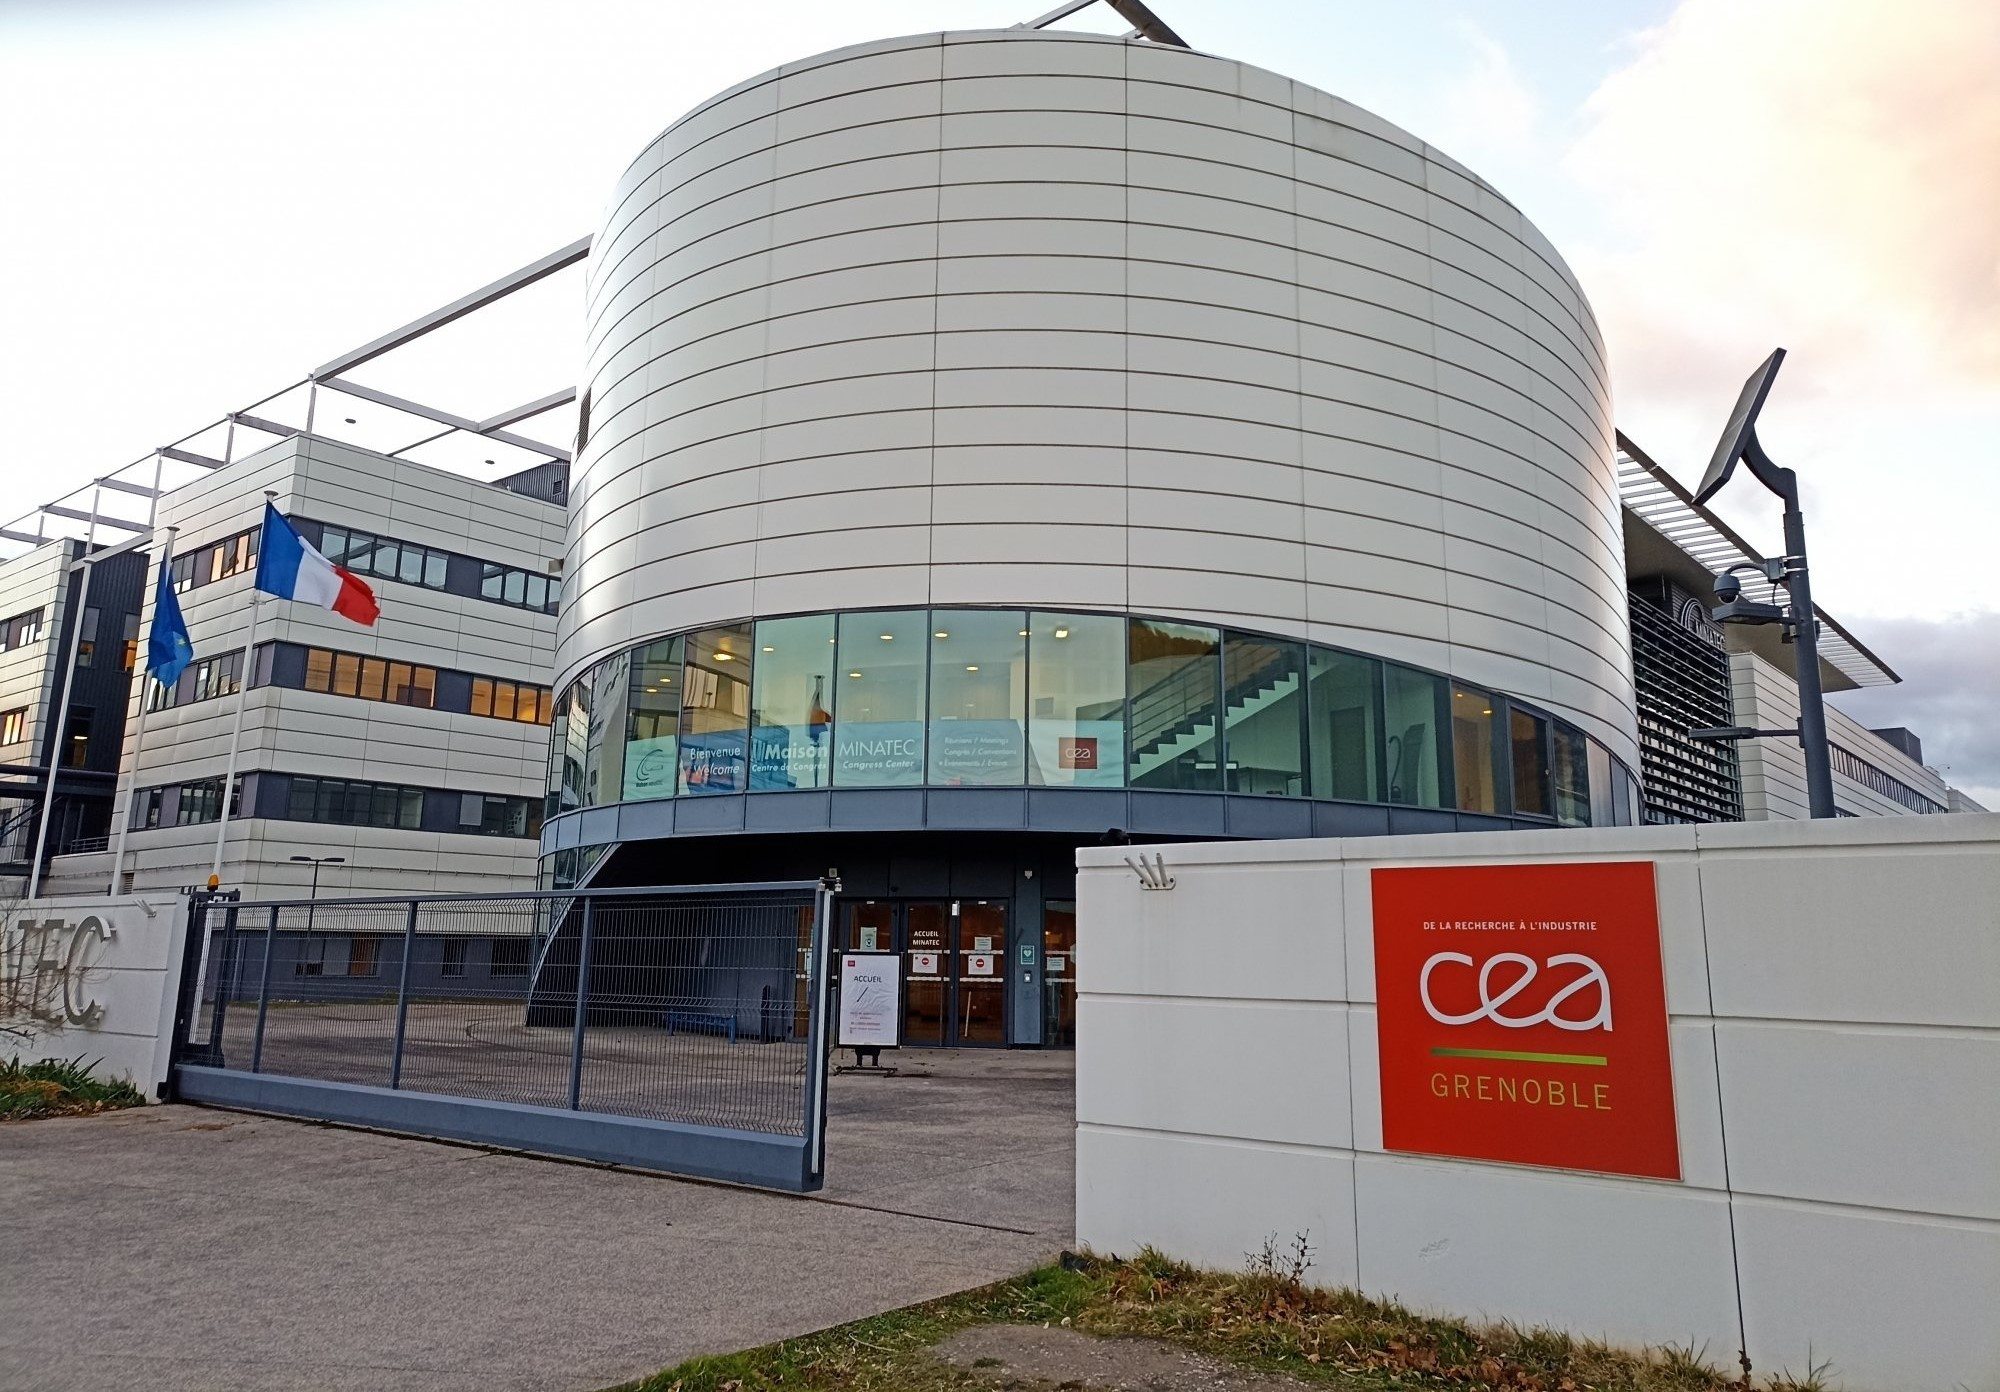
\includegraphics[width=0.8\textwidth]{images/ceaphoto.jpg}
    \caption{CEA Grenoble Campus}
\end{figure}

\FloatBarrier

\subsubsection{History}

\medskip

The French atomic energy commission, CEA, was born in 1945 after World War II. Its mission was to develop nuclear 
expertise for France. Pioneering scientists like Frédéric Joliot-Curie and Francis Perrin led the way in building 
research reactors and nuclear power plants.

\medskip

The CEA did not stop at just nuclear energy. In the 1960s, they began to diversify into new areas like renewable energy,
 micro and nanotechnologies, defense, and healthcare. This diversification led to the creation of specialized research
 centers, including the future innovation hub, CEA Grenoble.

\medskip

It was founded in 1956 by Nobel laureate physicist Louis Néel. He saw the scientific potential of the Grenoble
region and his vision proved to be true. The center grew rapidly in the following decades, attracting talent and investment
from around the world.

\medskip

It came to be known as France "atomic capital" due to its research reactors. However, their influence went far beyond
 nuclear. They developed their first integrated circuit in 1965, launching their journey into micro and nanotechnologies. 
 They also played a key role in creating Minatec, the first European hub for excellence in this field. In addition, they 
 became a leader in renewable energy research with the Institut national de l'énergie solaire (Ines).
 European synchrotron radiation facility (ESRF) was also established in Grenoble in 1988, further solidifying the city
 reputation as a scientific hub.
\medskip

Today, it is a research powerhouse with over 2,500 researchers and technicians. Their campus houses specialized
 institutes in various fields, from healthcare to digital technologies. It is also the headquarters for CEA Tech, the
 technological branch of the CEA with over 4,500 researchers across France.

\begin{figure}[h!]
    \centering
    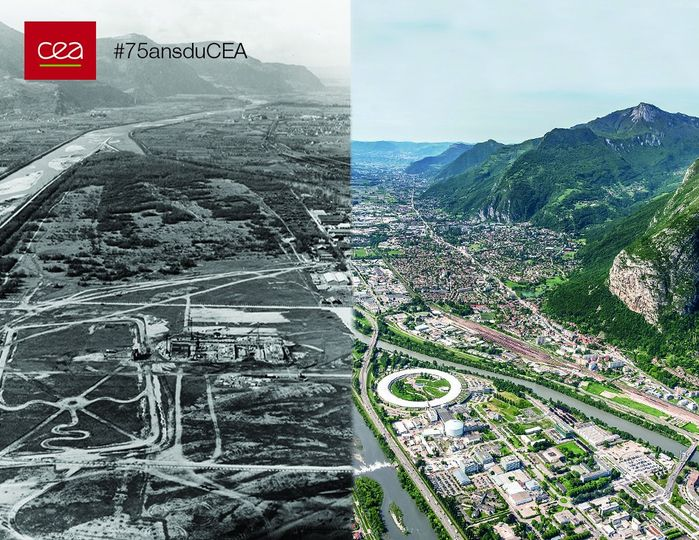
\includegraphics[width=0.8\textwidth]{images/old_new.jpg}
    \caption{CEA Grenoble campus before and after}
\end{figure}

\subsubsection{Sectors of activity}

CEA Grenoble plays a pivotal role in the nation economic and technological 
advancement through its groundbreaking research and innovations across diverse fields.

\begin{itemize}
  \item \textbf{Energy and Sustainability}: Supporting current and future nuclear power, exploring solar, hydrogen for carbon
  neutrality (2050), researching SMRs (Small modular reactors) and thermonuclear fusion.
  \item \textbf{Digital Technologies}: Contributing through the SPIN program for spintronic (frugal, agile, sustainable computing)
  aligned with France 2030 plan.
  \item \textbf{Healthcare}: Distinguished research in biology and biotechnology for health, addressing current and future challenges.
  (e.g., Laboratoire de biologie et biotechnologie pour la santé)
  \item \textbf{Defense}: Traditionally significant role, developing cutting-edge technologies for national security and defense 
  (less documented for Grenoble).
\end{itemize}

CEA Liten for example also serves as an innovation hub for new energy technologies and nanomaterials, emphasizing energy diversification
 and renewable energy integration. Their research encompasses solar photovoltaics, energy storage, and transportation (hydrogen and fuel
 cells).


\subsubsection{Future and orientation strategy}

\medskip

 CEA stands as a powerhouse for innovation in France.
 Spanning energy, healthcare, defense, and digital technologies, the CEA pushes boundaries by collaborating with universities
 and industry on ambitious R\&D projects.

\medskip

Their focus is clear: develop transformative solutions for global challenges. 
 This includes renewable energy sources, innovative healthcare systems, advanced defense solutions, 
 and disruptive digital technologies. Sustainability is paramount, with research prioritizing energy 
 efficiency and minimizing environmental impact.

\medskip

The CEA partners with leading institutions to accelerate technology transfer and create open innovation ecosystems. 
 These partnerships combine expertise, resources, and networks, leading to breakthrough technologies with significant 
 economic and social value.

\medskip

CEA Grenoble tries to prosper an innovative spirit. They focus on technologies like AI, advanced materials,
 nanotechnologies, and quantum technologies. Their research aims to improve industries, from
 developing next-generation batteries to creating innovative medical devices and advancing digital technologies.

\medskip

The challenges they tackle are various: climate change, the energy transition, emerging diseases, cybersecurity, and 
technological sovereignty. Their research is guided by a long-term vision, anticipating future challenges and preparing 
for them through innovation.

\medskip

The CEA aims to shape a sustainable future. They innovate in clean energy sources, 
advanced healthcare, robust national security, and a cutting-edge digital landscape. By working collaboratively and addressing
 global challenges head-on, the CEA tries to positions itself as a major contributor in the global scientific and technological landscape.

\medskip

\subsection{Project description}

\medskip
CEA Grenoble, a frontrunner in material metrology and characterization, recognizes the potential
 of CD-SAXS for analyzing nanostructures. To this end, CEA has actively invested in CD-SAXS development for several years.

\medskip

During my work-study program, I contributed to this initiative by developing a Python application
 for data fitting and analysis obtained through CD-SAXS. This technique relies on an inverse 
 algorithm that translates scattering intensity data into a relevant real-space structure. The 
 algorithm simulates the experiment using a model and iteratively compares the simulated data 
 with the experimental data until a good fit is achieved. A robust codebase is essential for 
 efficient CD-SAXS data processing.

\medskip

Previously, a collection of functions developed at CEA by former PhD students and at Lawrence Berkeley National Laboratory and Brookhaven National Laboratory served as the 
foundation for CD-SAXS analysis. However, it lacked the coherence of a well-structured application.
The code for various data simulation models was similarly disorganized. My primary task was to 
develop a user-friendly Python application that integrates these functions, streamlining data 
fitting and result analysis.

\medskip

Furthermore, the existing code suffered from slow execution speeds due to a lack of optimization.
To address this, I implemented optimizations and parallelization techniques, significantly 
improving the code efficiency.

\medskip


\subsection{Objectives}

\medskip

The initial aim of this project was commendable - to improve the existing CD-SAXS data analysis 
codebase. However, as we delved deeper, the project objectives evolved into a series of 
well-defined, targeted enhancements. This iterative approach ensured that our efforts addressed 
the specific needs of researchers at CEA Grenoble.

Here is a breakdown of the key objectives that emerged:

\begin{itemize}
    \item \textbf{Unleashing Computational Power:}
    \begin{itemize}
        \item \textbf{Vectorization for Server Optimization:} Standard code often struggles to fully leverage the parallel processing capabilities of modern servers. We identified the need to vectorize the code, allowing it to efficiently utilize the computational power available on CEA powerful servers. This significantly boosted the applications overall processing speed.
        \item \textbf{GPU Acceleration - Pushing the Limits:} Recognizing the ever-increasing capabilities of Graphics Processing Units (GPUs), we explored the potential of integrating GPU acceleration into the code. This would potentially unlock even faster performance, enabling us to tackle increasingly complex datasets.
    \end{itemize}
    \item \textbf{User-Centric Design:}
    \begin{itemize}
        \item \textbf{Building a Coherent Application:} The existing code, while functional, lacked the user-friendliness and intuitiveness necessary. We prioritized creating a well-structured, modular application. This would not only simplify data fitting and analysis but also make future feature additions and maintenance easier and more efficient.
        \item \textbf{Addition of different simulation models in the same codebase:} The original codebase had several independent simulation models: a model composed of stacked trapezoid, an overlay model and a rounded trapezoid model. We aimed to integrate these three models into a single, cohesive codebase. This consolidation would streamline the process of selecting and applying different models, enhancing the overall user experience.
      \end{itemize}
    \item \textbf{Quantifying Uncertainty - Confidence in Results:}
    \begin{itemize}
        \item \textbf{MCMC for Uncertainty Estimation:} A critical component missing from the original code was the ability to estimate the uncertainty associated with the fitted parameters. We addressed this by implementing a Markov Chain Monte Carlo (MCMC) algorithm. This powerful technique allowed us to generate a statistically representative set of solutions, enabling us to accurately estimate the level of uncertainty in the fitted parameters.
    \end{itemize}
    \item \textbf{Real-Time Uncertainty Estimation - Saving Valuable Time:}
    \begin{itemize}
        \item \textbf{On-the-Fly Uncertainty:} Taking the concept of uncertainty estimation further, we aimed to integrate this feature into the data acquisition process itself, specifically during synchrotron measurements. This would allow researchers to estimate the uncertainty in real-time. By setting a desired uncertainty threshold, the system could potentially stop the experiment once this level of certainty is achieved. This innovation has the potential to save valuable synchrotron beamtime, a precious resource for researchers.
    \end{itemize}
\end{itemize}

This refined set of objectives ensured that the project delivered valuable enhancements tailored to the needs of CEA researchers. The project not only improved the code performance but also transformed it into a user-friendly and powerful tool for analyzing CD-SAXS data with greater confidence.


\section{CD-SAXS}
\subsection{Introduction}

\medskip

Miniaturizing transistors, the building blocks of integrated circuits, is getting
tougher for the semiconductor industry. Shrinking their size and spacing (pitch)
brings not only manufacturing hurdles but also a metrology problem. Precisely
measuring these features during production is crucial for high-quality chips.
Existing in-line metrology techniques, like optical critical-dimension (OCD)
scatterometry and critical-dimension scanning electron microscopy (CD-SEM), are
nearing their limits \cite{SEM_resolution,OCD_resolution}. OCD struggles with limitations inherent to light and the
ever-shrinking features. CD-SEM offers valuable insights but is restricted by
the sampling area. To overcome these obstacles, the industry is exploring X-ray-based metrology.
X-rays have much shorter wavelengths than the features being measured, allowing
for more precise analysis. Additionally, they are sensitive to variations in
composition, providing a richer data set.

\medskip

Early research on X-ray characterization of patterned nanostructures used reflection
methods like X-ray diffraction (XRD) and grazing-incidence small-angle X-ray scattering (GISAXS). 
These techniques demonstrated X-ray's sensitivity to features' shape and spacing.
Furthermore, X-rays can probe buried features due to their sensitivity to composition via electron density. For instance, a GaInAs/InP multilayer was studied with high-resolution XRD, revealing 
sensitivity to both the grating and strain between layers \cite{Baumbach_Lübbert_Gailhanou_2000}.

\medskip

For sub-100 nm features, small-angle scattering methods like GISAXS become more practical. 
GISAXS examines nanostructures across large areas, making it a potential metrology tool 
for semiconductors. It uses X-rays near the critical angle of the probed film
resulting in a large sampling area and statistically significant data. This large area allows for faster measurements, enabling in situ kinetic studies.

\medskip

However, GISAXS limitations include a large spot size (50-100 mm wide by 5-10 mm long) and
computational challenges for complex nanostructure modeling. This limits its use for 
semiconductor metrology to simple, large-area patterns like memory arrays (Hofmann et al.,
2009; Scholze et al., 2011). Logic devices require smaller probing areas due to test structure 
size and the complexity of the multicomponent, 3D nanostructures. \cite{phd_freychet}

\medskip

Unlike other X-ray techniques, CDSAXS uses a transmission geometry, enabling a much smaller
spot size compared to methods like GISAXS. This allows for more precise measurements on smaller
features. Studies have shown CDSAXS's effectiveness in characterizing the shape and spacing of
nanometer-sized patterns \cite{sunday_2015}.

\medskip
CDSAXS  utilises variable-angle transmission scattering. By rotating the sample, it can probe the vertical profile of the nanostructures. This allows 
for reconstructing their shape and composition in two or even three dimensions.
We can think of it as a diffraction experiment for single crystals, but instead of a crystal, the 
periodic array of nanostructures acts like one. This technique excels at reconstructing 
intricate shapes smaller than 15 nm and with spacings around 30 nm, dimensions crucial for 
the semiconductor industry. \cite{first_cdsaxs_article}


\subsection{Experimental Setup}

During this project, I had the opportunity to work and observe how CDSAXS 
measurements are performed at the European Synchrotron Radiation Facility (ESRF)
in Grenoble, France. The ESRF is a world-renowned research facility that provides
intense X-ray beams for a wide range of scientific experiments. Specifically,
I worked with the BM02 beamline, which is dedicated to X-ray scattering and
   diffraction experiments.

\begin{figure}[h]
\centering
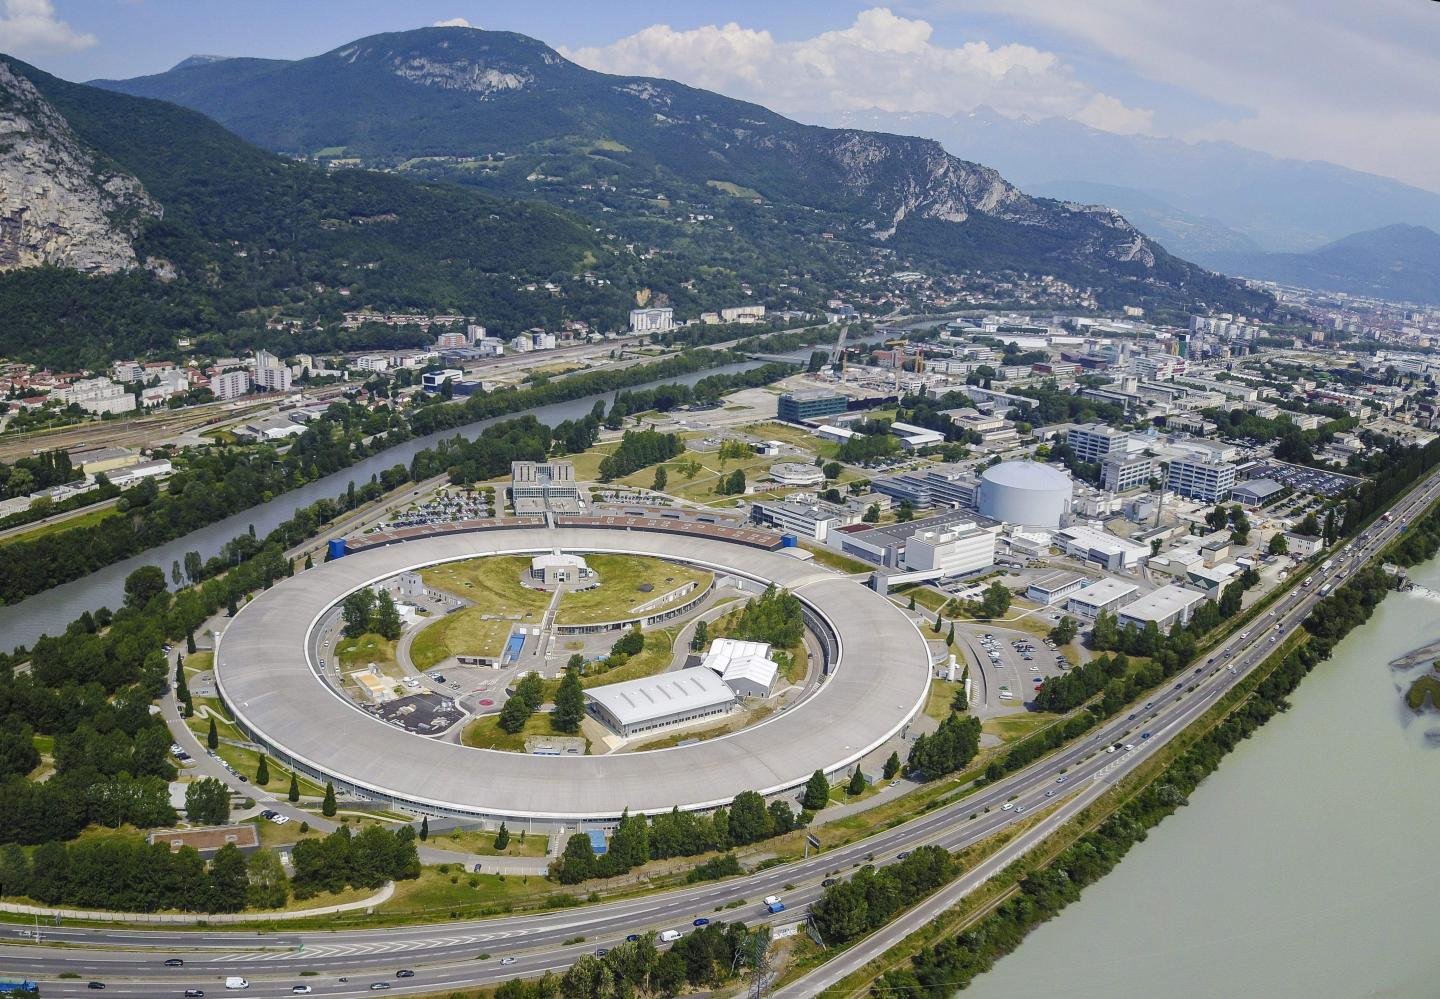
\includegraphics[width=0.6\textwidth]{images/esrf.jpg}
\caption{The European Synchrotron Radiation Facility (ESRF) in Grenoble, France. (credit: ESRF/Jocelyn Chavy)}
\label{fig
}
\end{figure}

The X-ray source obtained from the synchrotron is monochromatized and then focused using
various optical elements. The beam is then directed towards the sample. The 
sample is mounted on a device that allows for rotation and translation in all 
three dimensions. Once the alignment is complete, the sample is fixed in the
vertical direction and rotated in the horizontal plane, within a range of -60
to 60 degrees. The scattered X-rays are collected through a detector in a 
vacuum chamber. The schematic of the experiment is shown in Figure \ref{fig:exp_setup},
and the actual experimental setup is depicted in Figure \ref{fig:exp_setup_real}.

\medskip

One of the major challenges in the experiment is the alignment of the sample. 
Since the sample is rotated in the horizontal plane, it needs to be aligned 
such that the rotation axis is perpendicular to the beam. This is achieved by 
aiming a camera at the sample and focusing on the beam's position. A short 
measurement is then performed to observe the diffraction pattern of the sample.
 The rotation axis is adjusted until the diffraction pattern is horizontal and 
 centered.

\begin{figure}[h]
\centering
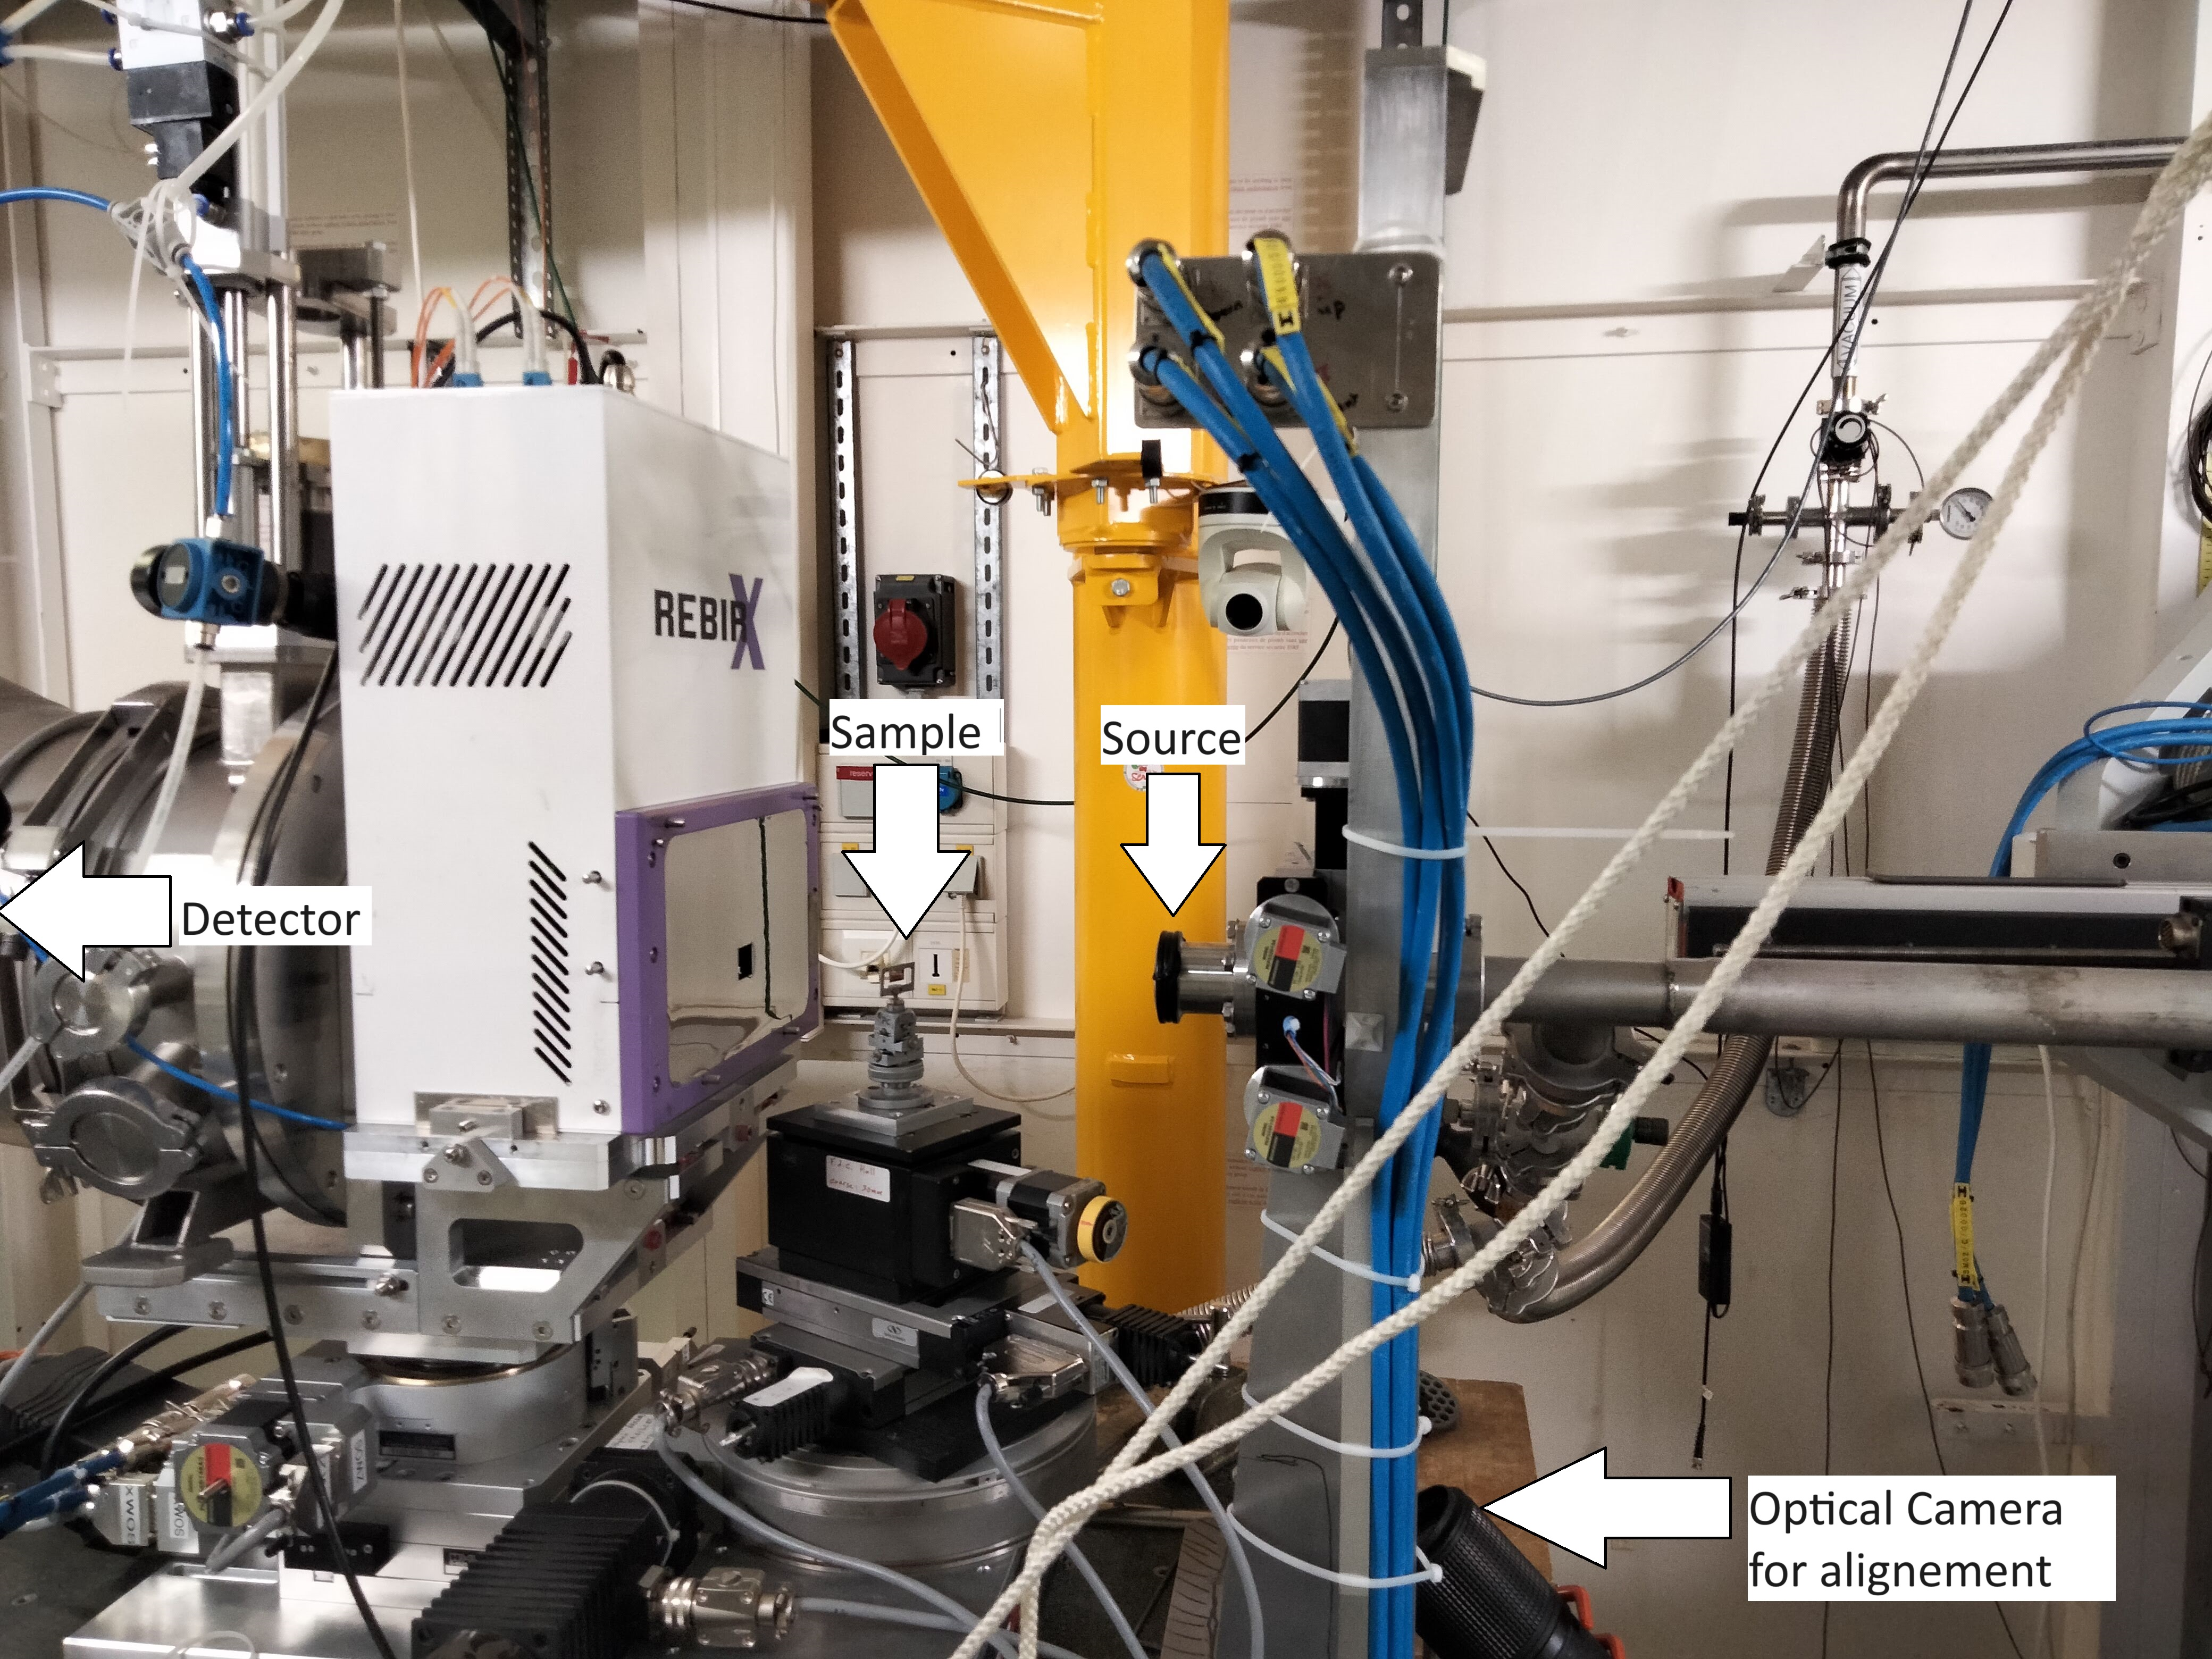
\includegraphics[width=0.6\textwidth]{images/photo_exp.jpg}
\caption{Picture of the experimental setup at the BM02 beamline at ESRF.}
\label{fig:exp_setup_real}
\end{figure}% talk about the alignement problem and how it was solved
\begin{figure}[h]
    \centering
    \begin{subfigure}[b]{0.8\textwidth}
        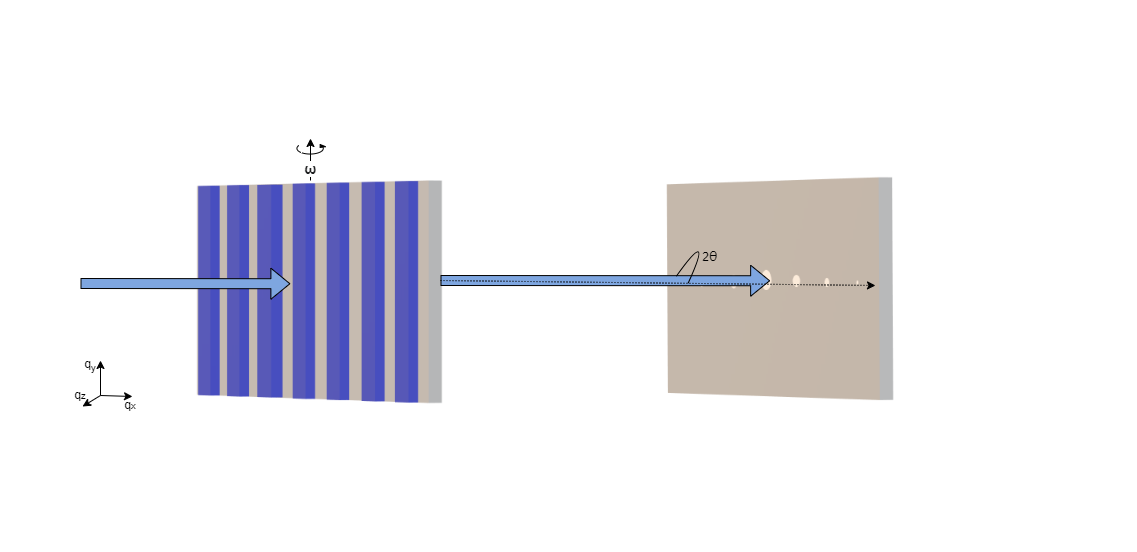
\includegraphics[width=\textwidth]{images/cdsaxs_diff.png}
        \caption{experimental setup}
        \label{fig:exp_setup}
    \end{subfigure}
    
    \begin{subfigure}[b]{0.4\textwidth}
        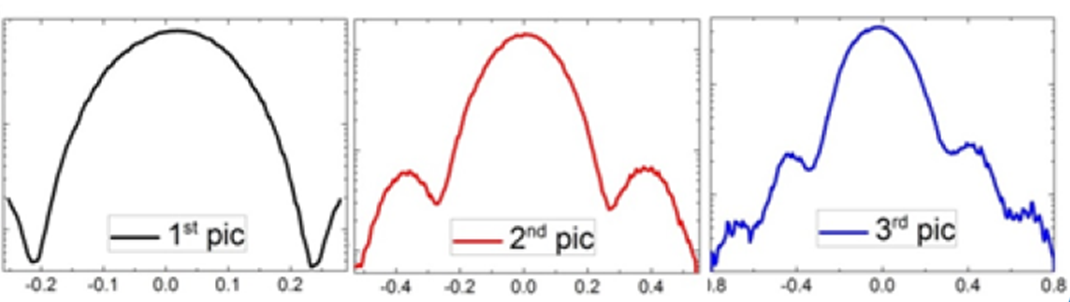
\includegraphics[width=\textwidth]{images/intensity_qz.png}
        \caption{Intensity vs $Q_z$}
    \end{subfigure}
    
    \caption{In a is the schematic of the CD-SAXS instrument layout. The X-ray beam (thick solid lines) is transmitted through the 
    patterned sample. Scattered intensity (I) is measured by a 2D detector as a function of scattering angle $(2\theta)$ 
    and converted to $I(Q_{x})$, where $Q_{x}$ is defined in the text. Measurements are performed at various sample incidence 
    angles $(\theta')$. In b After conversion from the $(Q_{x},\omega)$
    plane, the intensities
   from a trapezoidal cross section would appear as predicted in
   the model calculation on b, plotted as I as a function of the
   Fourier component, $Q_{Z}$.}
   \label{fig:isolated_line}
\end{figure}

\FloatBarrier

\subsection{Scattering Model} \label{sec:scattering_model}

\medskip
We can represent the diffraction of a collimated X-ray beam by:

\begin{equation}
    I(\mathbf{Q}) = \varOmega | F(\mathbf{Q}) |^2,
\end{equation}
    
where $I(\mathbf{Q})$ represents the scattered intensity as a function of the scattering
vector $\mathbf{Q}$, $\mathcal{F}$ is a constant independent of $\mathbf{Q}$,
and $F(\mathbf{Q})$ is the Fourier transform of a function describing the mass
distribution within the nanoimprinted pattern. 
    
This relationship is considered valid within the limitations of the CDSAXS geometry,
which includes a transmission geometry and a low probability of multiple scattering.    
Unfortunately, the conjugate product in the equation leads to a loss of phase
information, making it impossible to analytically extract $F(\mathbf{Q})$ from $I(\mathbf{Q})$.
Therefore, the primary method for determining feature dimensions involves constructing
a real-space model of the pattern's cross-section. The Fourier transform of this 
model is then fitted to the experimental CDSAXS data.

\medskip

During my work-study program, we were mainly concerned with lines of nanostructures (see figure \ref{fig:isolated_line}). The cross-section of
these can be represented as a stack of trapezoids.
\begin{figure}[h]
    \centering
    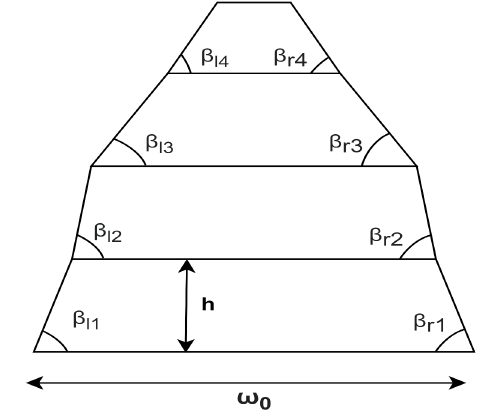
\includegraphics[width=0.2\textwidth]{images/trapezoid.png}
    \label{fig:trapezoid_model}
    \caption{Cross-section of a nanostructure line represented as a stack of trapezoids.}
    
\end{figure}
We can calculate the analytical fourier transform of a trapezoidal shape to use for fitting
can be calculated is given by expression \cite{sunday_2015}:
\begin{equation}
    F\left(q_{x}, q_{z}\right)=\frac{1}{q_{x}}\left[-\frac{m_{1}}{t_{1}} e^{-i q_{x}\left(\frac{\omega_{0}}{2}\right)}\left(1-e^{-i h\left(\frac{q_{x}}{m_{1}}+q_{z}\right)}\right)\right. \\ +\frac{m_{2}}{t_{2}} e^{-i q_{x}\left(\frac{\omega_{0}}{2}\right)}\left(1-e^{\left.-i h\left(\frac{q_{x}}{m_{2}}+q_{z}\right)\right)}\right]
    \label{eq:trapezoidal_ft}
\end{equation}
where,

\( \begin{array}{l}\mathrm{m}_{1}=\tan \left(\beta_{1}\right) , m_{2}=\tan \left(\pi-\beta_{r}\right), \\ t_{1}= q_{x}+m_{1} q_{z}, t_{2}= q_{x}+m_{2} q_{z}\end{array} \)

\medskip

so,
\begin{equation}
    I_{0}(\mathbf{q}) = |F(q)|^{2}
\end{equation}

An additional decay of scattered intensity $I(Q_{x})$ is expected beyond that predicted by the trapezoidal model.
This arises from the distribution of periodicities within the sample. This distribution 
can be caused by two factors:
\begin{itemize}
    \item \textbf{Random variations in average line position}: In this case, the line width remains
         constant, but the average position of the lines fluctuates slightly across the 
         sample.
    \item \textbf{Variations in line width}: Here, the line width itself varies, 
        which also affects the periodicity.
\end{itemize}

Both factors indicate a degree of long-range order within the pattern. Additionally, they provide insights into specific types of line edge roughness \cite{these_reche}.

To account for this distribution, we introduce an effective Debye-Waller factor, similar to the one used for fluctuations in crystal lattices.

Hence,

\begin{equation}
    I(\mathbf{q}) = I_{0}(\mathbf{q}) \exp(-q^{2}DW^{2} )
\end{equation}

where $DW$ is the Debye-Waller factor.

\subsection{Fitting Algorithm}

While CDSAXS excels at detecting deviations from a perfect grating pattern in buried structures, it requires additional processing to convert the raw data into a meaningful real-world structure. This process involves using an inverse algorithm, which essentially translates the scattered intensity information back into the original structure's characteristics.

\medskip

However, there's a catch. Traditional optimization methods used for refinement often fall short when dealing with complex internal structures with numerous parameters. These methods rely on iteratively simulating scattering data and comparing it to the measured data. Unfortunately, this approach can be very time-consuming, especially for intricate structures.

\medskip

Another challenge arises from the possibility of "degenerate" solutions. These occur when multiple structural models can produce the same scattering data, making it difficult to pinpoint the true structure. This is a common issue in scattering analysis.

\medskip

Therefore, the ideal scenario for CDSAXS analysis involves an optimization algorithm that can consistently and rapidly converge on the best possible fit for the data. While some prior knowledge about the underlying structure can accelerate the process, such information isn't always readily available. This highlights the need for more efficient algorithms that can handle complex structures even with limited prior knowledge.

\medskip

Previous research has explored various algorithms to determine the optimal set of parameters for a model that best fits the measured CDSAXS data. These parameters essentially describe the actual structure of the nanostructure being analyzed.

\medskip

One approach utilizes a Markov chain Monte Carlo (MCMC) algorithm. However, this method requires a good initial guess for the structure's parameters and limitations on their search range. Additionally, it necessitates multiple independent runs to ensure the algorithm converges on the correct solution. While this approach can be effective, the need for tight parameter bounds might overlook potential fabrication errors in the sample.

\medskip

Another strategy involves massive computing resources with parallelization and highly refined grid-based models. This method, known as reverse MCMC, offers greater accuracy but is limited by the availability of such computational power.

\medskip

Genetic and evolutionary algorithms have emerged as promising alternatives. These methods mimic biological evolution, with the model parameters acting as the "genetic code." Starting with randomly generated parameters, these algorithms iteratively refine them through a "mixing strategy" over multiple generations until the optimal set is found. This approach excels at searching large parameter spaces with wide bounds, making it suitable for complex structures.
\cite{hannon2016advancing}
\subsubsection{Covariance Matrix Adaptation Evolution Strategy (CMAES)}

One such algorithm is the Covariance Matrix Adaptation Evolution Strategy (CMAES). This method is particularly well-suited for high-dimensional optimization problems, making it ideal for complex nanostructure analysis. CMAES operates by maintaining a population of candidate solutions, with each iteration generating new candidates based on the previous generation's performance. By adapting the covariance matrix of the candidate solutions, CMAES can efficiently explore the parameter space and converge on the optimal solution.

\begin{figure}[h]
    \centering
    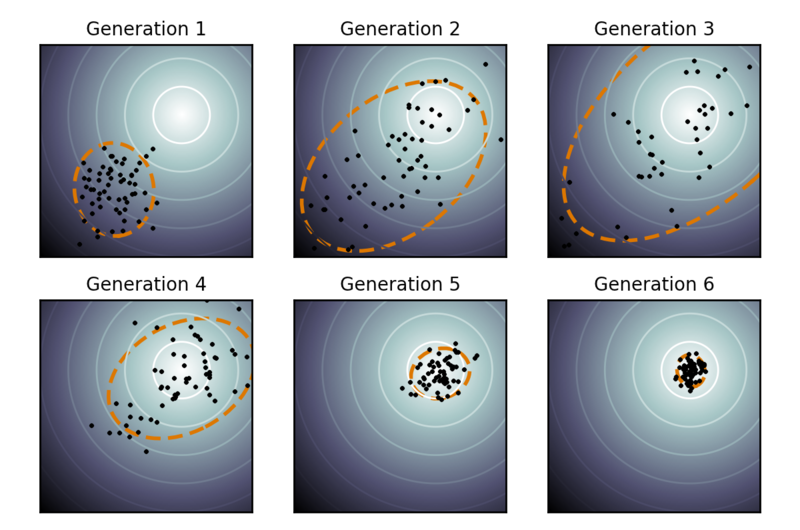
\includegraphics[width=0.8\textwidth]{images/CMAES.png}
    \caption{Illustraion of CMAES algorithm. The algorithm maintains a population of candidate solutions, with each iteration generating new candidates based on the previous generation's performance.(image taken from wikipedia CMAES page) }
    \label{fig:cmaes}
\end{figure}

\FloatBarrier

\medskip

The code for CD-SAXS generates a set of possible solutions for the parametres of the model. Then we calculate the 
analytical fourier transform of the model and compare it with the experimental data. To compare the two,
we use mean-absolute error log:

\medskip

\begin{equation}
    \Xi=\frac{1}{N_{\mathrm{q}}-1} \sum_{\mathbf{q}}\left|\log _{10} I_{\mathrm{Sim}}(\mathbf{q})-\log _{10} I(\mathbf{q})\right|
\end{equation}

\medskip

where $I_{\mathrm{Sim}}(\mathbf{q})$ is the simulated intensity and $I(\mathbf{q})$ is the experimental intensity.

\medskip

We call it the goodness of fit. The algorithm then tries to minimize this quantity by adjusting the parameters of the model.

\medskip

In an article \cite{hannon2016advancing}, researchers investigated the efficiency of various algorithms
for reconstructing various nanostructures using X-ray scattering data.
Their findings specifically highlighted the advantages of the CMAES. Compared to other
methods like Markov Chain Monte Carlo (MCMC) and Differential Evolution 
(DE), CMAES demonstrated significantly faster convergence times when 
analyzing an experimental structure. Notably, CMAES achieved a solution 
that matched the quality of previous studies in approximately 1 to 2 
orders of magnitude less time than MCMC and less than an order of 
magnitude time than DE. This speed advantage held true regardless 
of the specific objective function used to evaluate the goodness of fit. 
These results suggest that CMAES offers a powerful tool for analyzing 
complex nanostructures with X-ray scattering data, particularly when 
dealing with limited computational resources or tight time constraints.

\subsubsection{Uncertainity estimation by Monte Carlo Markov Chain(MCMC) method}
\label{sec:mcmc_cdsaxs}

The CMAES algorithm provides a single best-fit solution for the nanostructure parameters. However, it's essential to understand the uncertainty associated with these parameters.
This uncertainity relates to the different possible combinations of parameters that could result in a similar goodness of fit. 
For instance, decreasing slightly height of one trapezoid and increasing the height of other one can result in a similar goodness of fit.
To address this, we can use MCMC algorithm to explore and find all the sets of population that can result in the same goodness of fit.

\medskip

This confidence interval then can be calculated from this population of parameters. This interval gives us an idea of the range of possible values for each parameter that could still provide a good fit to the data.
The lower and upper bounds of this interval can be used to estimate the uncertainty associated with each parameter.

\begin{figure}[h]
    \centering
    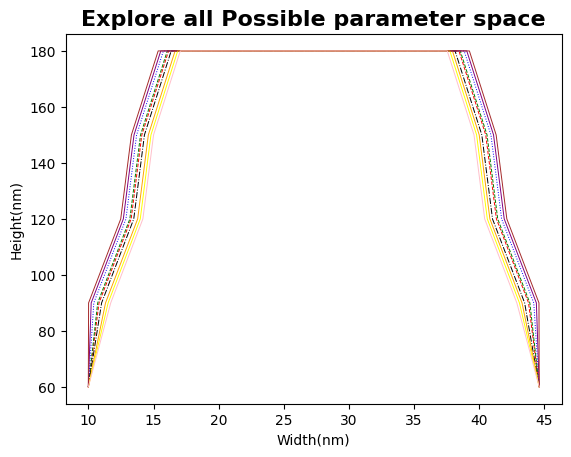
\includegraphics[width=0.5\textwidth]{images/mcmc.png}
    \caption{MCMC algorithm exploring all possible sets of parameters that can result in the same goodness of fit.}
\end{figure}
\medskip

After determining the best-fit model structure, the researchers of this article \cite{sunday2016evaluation}
employed a MCMC algorithm to calculate the uncertainties associated with the model parameters.
This algorithm generates a population of models that can be evaluated to assess the uncertainty
in a set of parameters. The probability of a given model being accepted into the population
depends on how well the simulated scattering profile it generates matches the experimentally
measured one.

Here is the overview of there algorithm:

\begin{enumerate}
    \item \textbf{Seeding:} The algorithm initializes with the model (M) exhibiting the best known goodness-of-fit, denoted GFB.
    \item \textbf{Proposal generation:} Random perturbations are applied to each parameter within the model, resulting in a new candidate model (M$_i$) and its corresponding goodness-of-fit GF (GF$_i$).
    \item \textbf{Acceptance for better fit:} If GF$_i$ $<$ GF$_{i-1}$, then M$_i$ is automatically accepted into the population (and GFB is updated to GFB = GF$_i$ if the new model has a better fit).
    \item \textbf{Metropolis-Hastings acceptance for worse fit:} If GF$_i$ $>$ GF$_{i-1}$, the probability (P$_i$) of accepting M$_i$ is calculated using Eq. \eqref{eq:mcmc_acceptance}:
    \begin{equation}
        P_i = \exp \left( -0.5 \cdot (\text{GF}_i - \text{GFB}) \right) \label{eq:mcmc_acceptance}
    \end{equation}
    A random number $\alpha$ between 0 and 1 is then generated. If $\alpha < P_i$, M$_i$ is accepted; otherwise, it is rejected, and a new proposal is generated from M$_{i-1}$.
    \item \textbf{Equilibrium and resampling:} Steps 2-4 are repeated until the model population reaches equilibrium. To avoid correlations between accepted models, the population is resampled (e.g., every 50 steps in this case).
    \item \textbf{Uncertainty calculation:} The uncertainties are calculated from the final accepted model population and represent 95\% confidence intervals. The step size for generating proposals was optimized to achieve an
     acceptance probability between 0.25 and 0.35, a range known to yield the fastest convergence.
\end{enumerate}

I used a very similar algorithm but with some modifications to increase the efficiency, we will discuss this in the next section.

\subsubsection{Overall view}

\medskip

The process begins with an initial guess for the parameters of the model, which describe a geometric structure with specific width and height parameters. The model data is then transformed into the frequency domain using a Fourier Transform, and this transformed data is compared with the experimental data to optimize the fit by adjusting the parameters and reducing the error between the simulated and experimental data.

\medskip

The error between the experimental and simulated data is quantified using an error metric that measures the goodness-of-fit by comparing the logarithms of the simulated and experimental intensity profiles. If the error is within a tolerable range, the fit is considered acceptable, and the best-fit model is extracted. This involves identifying the parameters that provide the best match to the experimental data.

\medskip

To quantify the uncertainties associated with the fitted parameters, a Monte Carlo approach is employed. This involves exploring the possible parameter space through a series of stochastic simulations. The MCMC method is used to sample the parameter space, ensuring that the distribution of the sampled parameters reflects their likelihood given the data. During the MCMC process, initial samples are generated from the best-fit parameters, new samples are proposed by perturbing the current parameters, and the Metropolis-Hastings criterion is used to decide whether to accept or reject the new samples based on their goodness-of-fit compared to the previous samples. This process is repeated until a sufficient number of samples are collected, ensuring the sampled parameter distribution converges to the true posterior distribution.

\medskip

The final step involves calculating the error bars (uncertainties) for the fitted parameters based on the Monte Carlo samples, providing 95\% confidence intervals and a robust measure of the reliability of the fitted model parameters. By combining CMAES for initial parameter optimization and MCMC for uncertainty quantification, the algorithm offers a robust approach to model fitting, ensuring both optimal parameter estimation and reliable uncertainty analysis.

\medskip

Here is a figure that shows the overall view of the CD-SAXS algorithm:

\begin{figure}[h]
    \centering
    \begin{subfigure}[b]{1\textwidth}
        \centering
        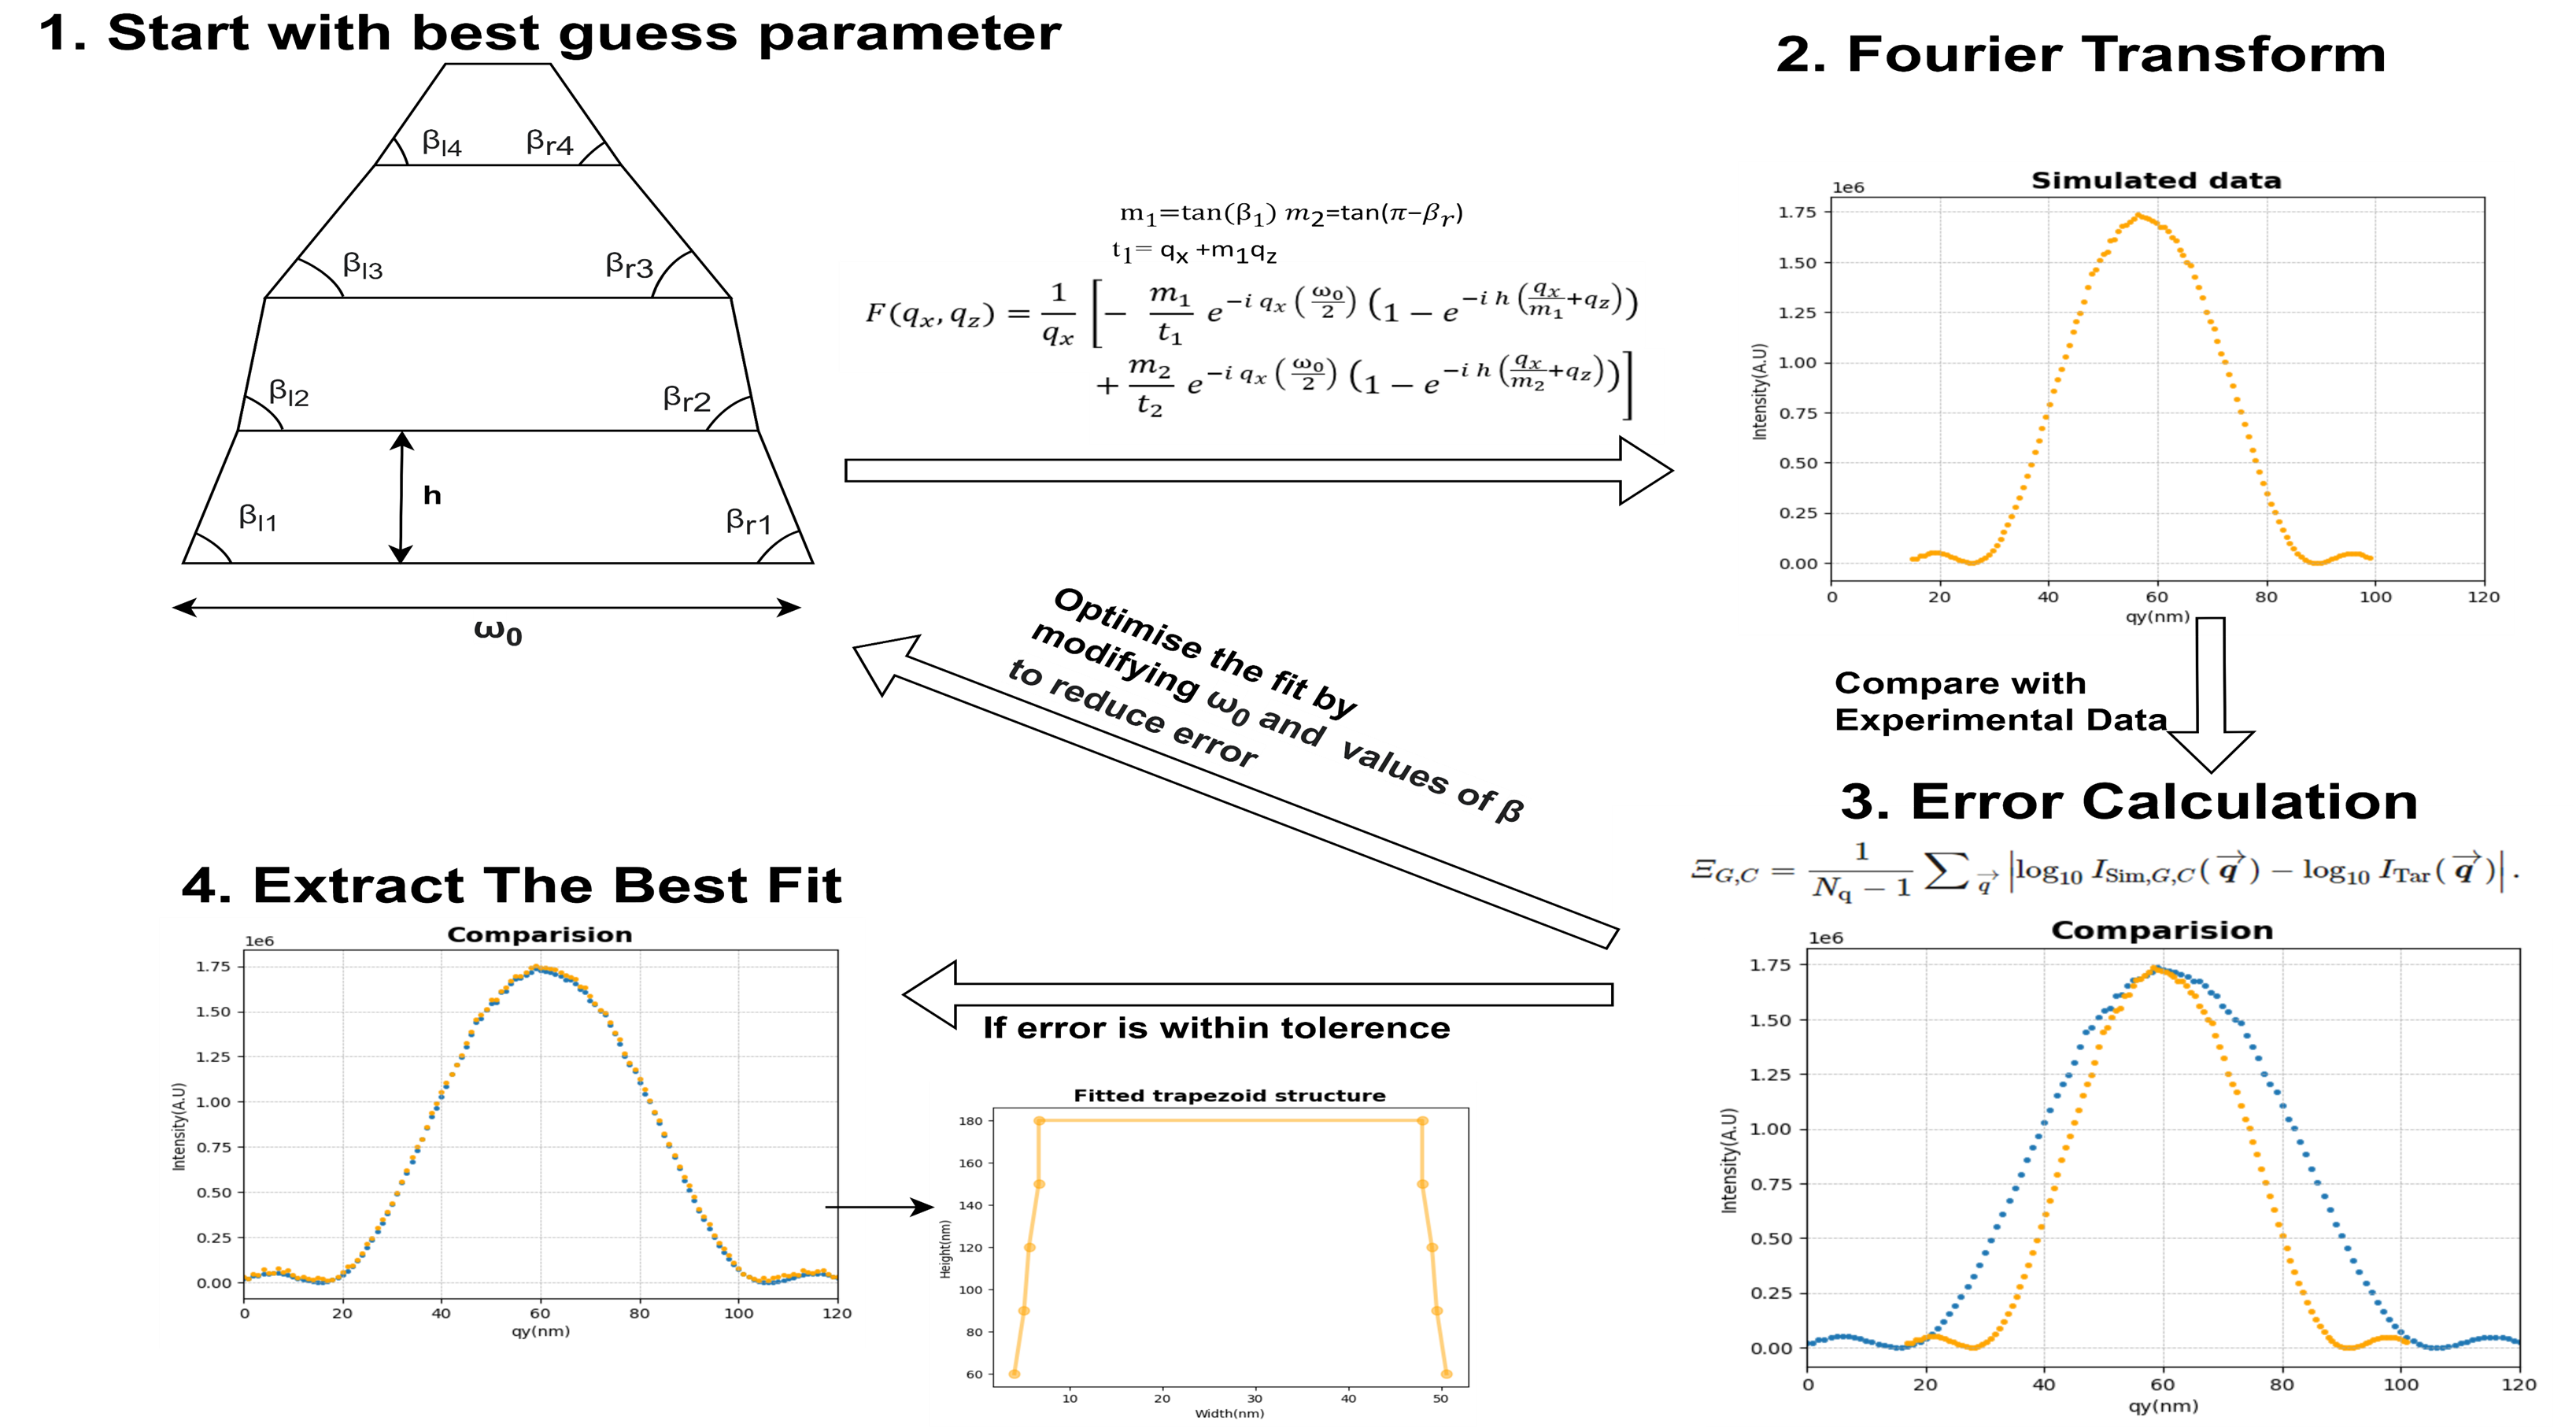
\includegraphics[width=\textwidth]{images/cmaes_overall.png}
    \end{subfigure}
    \\
    \begin{subfigure}[b]{1\textwidth}
        \centering
        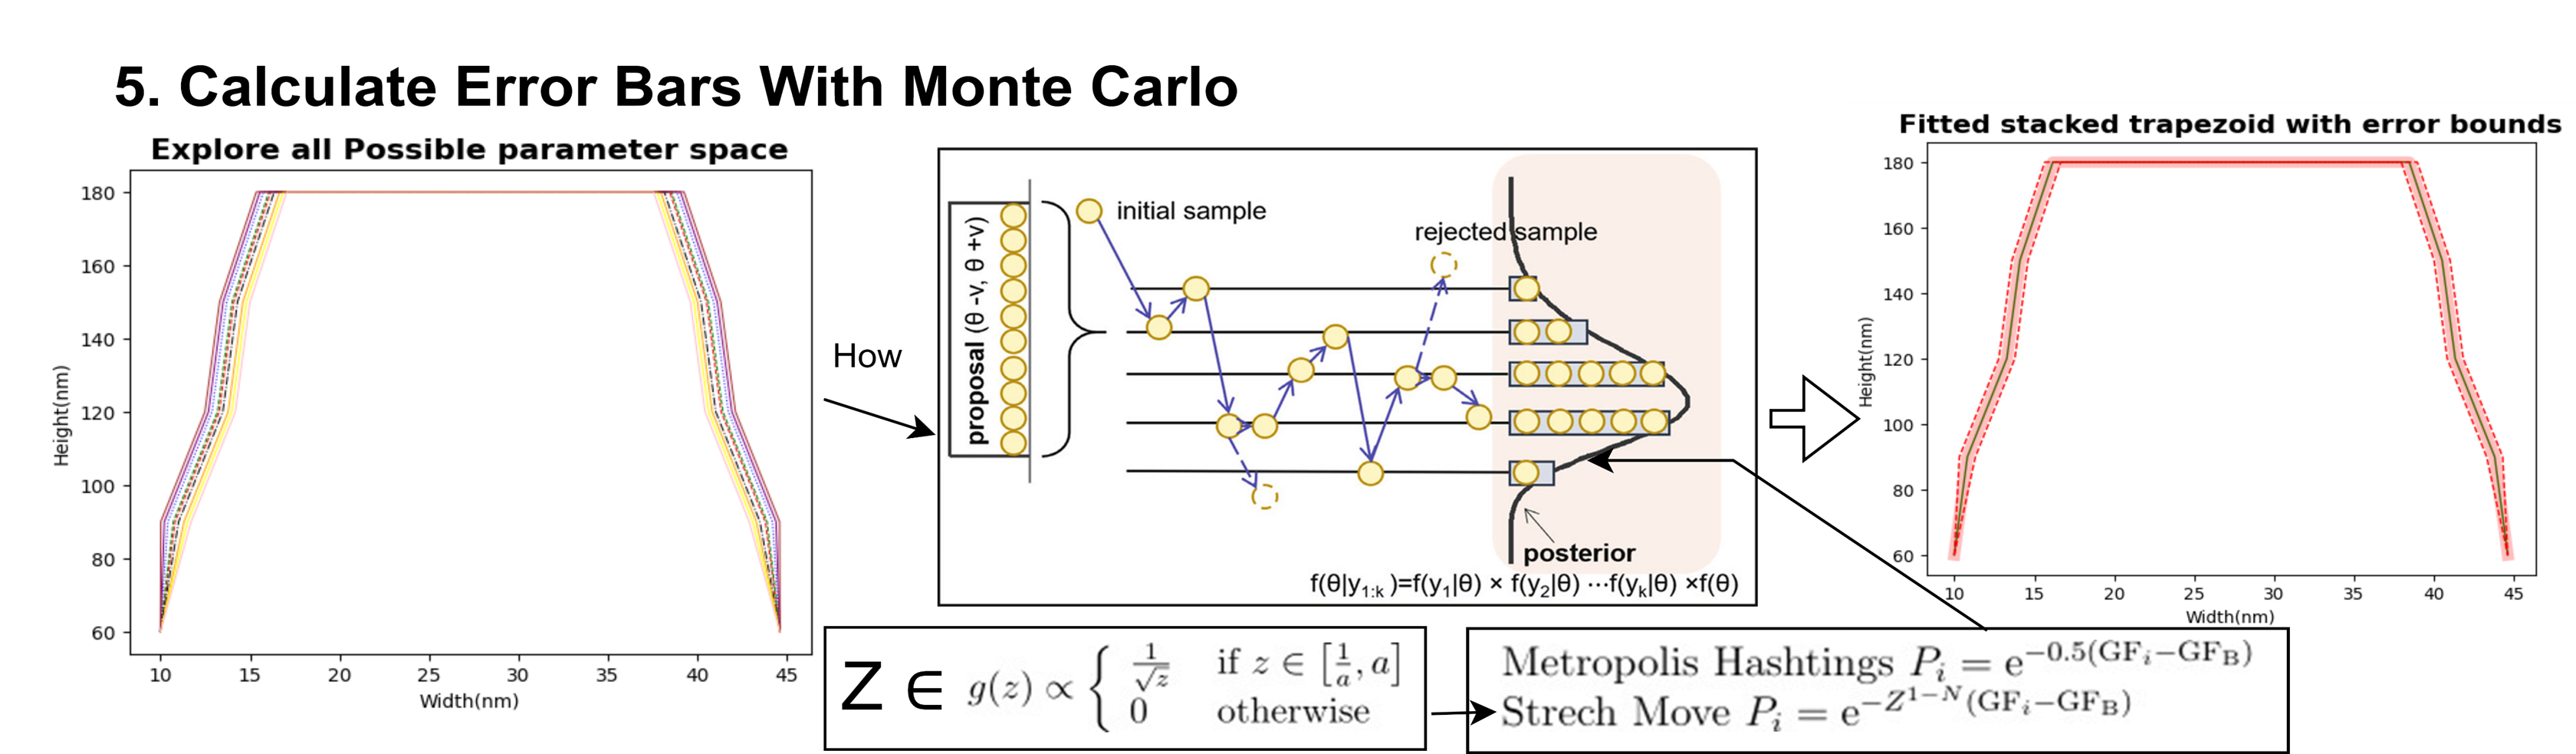
\includegraphics[width=\textwidth]{images/mcmc_overall.png}
    \end{subfigure}
    \caption{This algorithm integrates CMAES for initial parameter optimization and MCMC for uncertainty quantification. By combining these methods, the algorithm provides a robust approach to model fitting, ensuring both optimal parameter estimation and reliable uncertainty analysis.}
    \label{fig:cd_saxs_algo}
\end{figure}

\FloatBarrier




\section{CD-SAXS Python Application}
\subsection{Introduction}
\subsection{Conception}
\subsection{Simulation Models}
\subsection{On the fly uncertainity estimation}
\subsection{Future Prospects}

\newpage

%generate the bibliography
\printbibliography

\end{document}
